\scanpage{27}
% archive sheet number: 26

cette dernière relation $\Sigma_1^-\cap\Sigma_2^-\ne\varnothing$ est vraie $=$ si $E_1=E_2=\varnothing$, car \deleted{\unsure{alors} par hyp.} si on avait de plus $\Sigma_1^-\cap\Sigma_2^-=\varnothing$, on en conclurait que les deux \deleted{part.} décompositions binaires \deleted{\unsure{son|se}} (qui sont \unsure{alors|donc} des partitions binaires) sont \uline{identiques}, ce que l'on \inserted{a} exclu. Cela montre que les $\Sigma_1^+,\Sigma_2^+$ sont uniquement déterminés.

On a donc le diagramme d'inclusions
\diagram{\begin{tikzcd}[ampersand replacement=\&,column sep=small]
\Sigma_1^+ \& E_1 \arrow[l,hook] \arrow[r,hook] \& \Sigma_{12} \& E_2 \arrow[l,hook] \arrow[r,hook] \& \Sigma_2^+
\end{tikzcd}}
qu'on, exprime par un diagramme
\figure{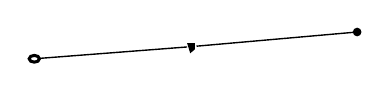
\begin{tikzpicture}[x=1cm,y=1cm]
\draw[line width=0.5pt] (0,0) -- (1.94,0.15);
\draw[line width=0.5pt] (2.06,0.16) -- (4.10,0.34);
\draw[fill=white,line width=1.1pt] (0,0) ellipse[x radius=0.065,y radius=0.043];
\fill (1.94,0.20) -- (2.04,0.20) -- (2.04,0.12) -- (1.98,0.07) -- cycle;
\fill (4.10,0.34) circle[radius=0.055];
\end{tikzpicture}}
\diagram{\begin{tikzcd}[ampersand replacement=\&,column sep=small]
\Sigma_1^+ \& E_1 \arrow[l,hook] \arrow[r,hook] \& \Sigma_{12} \& E_2 \arrow[l,hook] \arrow[r,hook] \& \Sigma_2^+
\end{tikzcd}}
\margin{\[
\text{NB}\left\{\begin{aligned}
\Sigma_1^-&=\Sigma_{12}\amalg_{E_2}\Sigma_2^+\\
\Sigma_{\deleted{\unsure{1}}2}^-&=\deleted{E}\Sigma_{12}\amalg_{E_1}\Sigma_1^+
\end{aligned}\right.
\]}

\margin{Ceci n'implique pas que les quatre ensembles $\Sigma_1^+,\Sigma_1^-,\Sigma_2^+,\Sigma_2^-$ soient distincts, car on peut avoir (non pas $\Sigma_1^+=\Sigma_2^+$, ni $\Sigma_1^-=\Sigma_2^-$, mais) $\Sigma_1^+=\Sigma_2^-$, qui équivaut à $E_1=\Sigma_{12}$ et entraîne $E_2=\varnothing$
(Cela signifie, en termes des $(\Sigma_1^+,\Sigma_1^-)$ que $\Sigma_2^{\unsure{\dot{-}|-}}=\Sigma_1^+$, $\Sigma_2^+=X\setminus\Sigma_1^+=\overset{\unsure{\circ|\leftarrow}}{\Sigma}{}_1^{-,\unsure{\circ|0}}$) \deleted{\unsure{ou}} et la relation \unsure{symetrique|symétrique}. On ne veut pas exclure ce cas, i.e.\ \deleted{\unsure{mais|nous}} n'exige pas que les quatre ensembles $\Sigma_1^+,\Sigma_1^-,\Sigma_2^+,\Sigma_2^-$ soient distincts s'ils le \unsure{\deleted{sont}|sont}, on dit que les \deleted{ens.} \inserted{deux décomp. bin.} \deleted{\unsure{sont strictmt}} non parallèles.}

Je me propose d'étudier les ensembles finis \unsure{indicellés|indiciellés|indécollés|indécollt} $\deleted{\unsure{\Pi|\Sigma}}(\Pi_\alpha)_{\alpha\in A}\deleted{=(\unsure{\Sigma_\alpha^i}),\unsure{\alpha\in A}}$
$\deleted{\unsure{\pi_\alpha|\Pi_\alpha}=\{\Sigma_\alpha^\varepsilon}$ \unsure{de|des} décompositions binaires de $\unsure{X}$ deux à deux non parallèles.

Voici une façon \unsure{très|\deleted{très}} \unsure{générale|génerale} d'\deleted{\unsure{en}}obtenir des floppées.
